\chapter{Introduction}
\label{c.intro}

\section{The Epoch of Reionization}

Our Universe has a complex, rich history, of which enormous progress has been made in the past few decades to unravel its story. Much has been learned about the very beginnings of the Universe, from the Big Bang's large explosion of energy to the relatively smooth and simple cosmic background radiation that was leftover. Additionally, observational feats have revealed the status of the present-day Universe and the intricate \textit{cosmic web}, or large scale structure, of galaxies today. 

The Epoch of Reionization (EoR) ties these two bookends together, occurring about a billion years after the Big Bang when the very first stars and galaxies formed. How did the tiny density fluctuations from the cosmic microwave background develop into the structure we see today? How did the first luminous structures form, and how did they evolve and influence the gas around them? Exploring the reionization era opens up a new chapter of our Universe's story - a chapter that promises to connect the dots between our past and present.

\subsection{Cosmic History}

As the Universe expanded and cooled after the Big Bang, electrons and protons eventually combined to form neutral hydrogen atoms. At the young age of $\sim$ $380,000$ years, the Universe's ordinary baryonic content was almost entirely neutral hydrogen, while most of its total matter was dark matter (\citealt{loeb_furlanetto_2013}). Then, for the next several hundred million years, the \textit{Dark Ages} proceeded, with concentrations of dark matter setting the foundations for the formation of the first luminous structures. More specifically, the tiny, primordial density fluctuations that were established at the release of the CMB grew with inflation and the expansion of the Universe. The densest regions then collapsed to form dark matter halos, inside of which hydrogen gas could cool, condense, and fragment into stars (\citealt{dodelson_cosmology}).

The first luminous structures are thought to have formed at an age of $\sim$ $200$ million years (z $\sim$ 20) and are predicted to have been massive stars with high luminosities and large ionizing powers (\citealt{loeb_furlanetto_2013}). The ionizing photons from the first stars carved out pockets of ionized hydrogen gas, and as the number of sources grew, an increased number of ionized bubbles emerged. Eventually, the first generations of stars and galaxies are responsible for ionizing all the neutral hydrogen in the Universe, with reionization complete by about one billion years after the Big Bang (z $\sim$ 6) (\citealt{furlanetto_et_al2006}). 

\begin{figure}
	\centering
	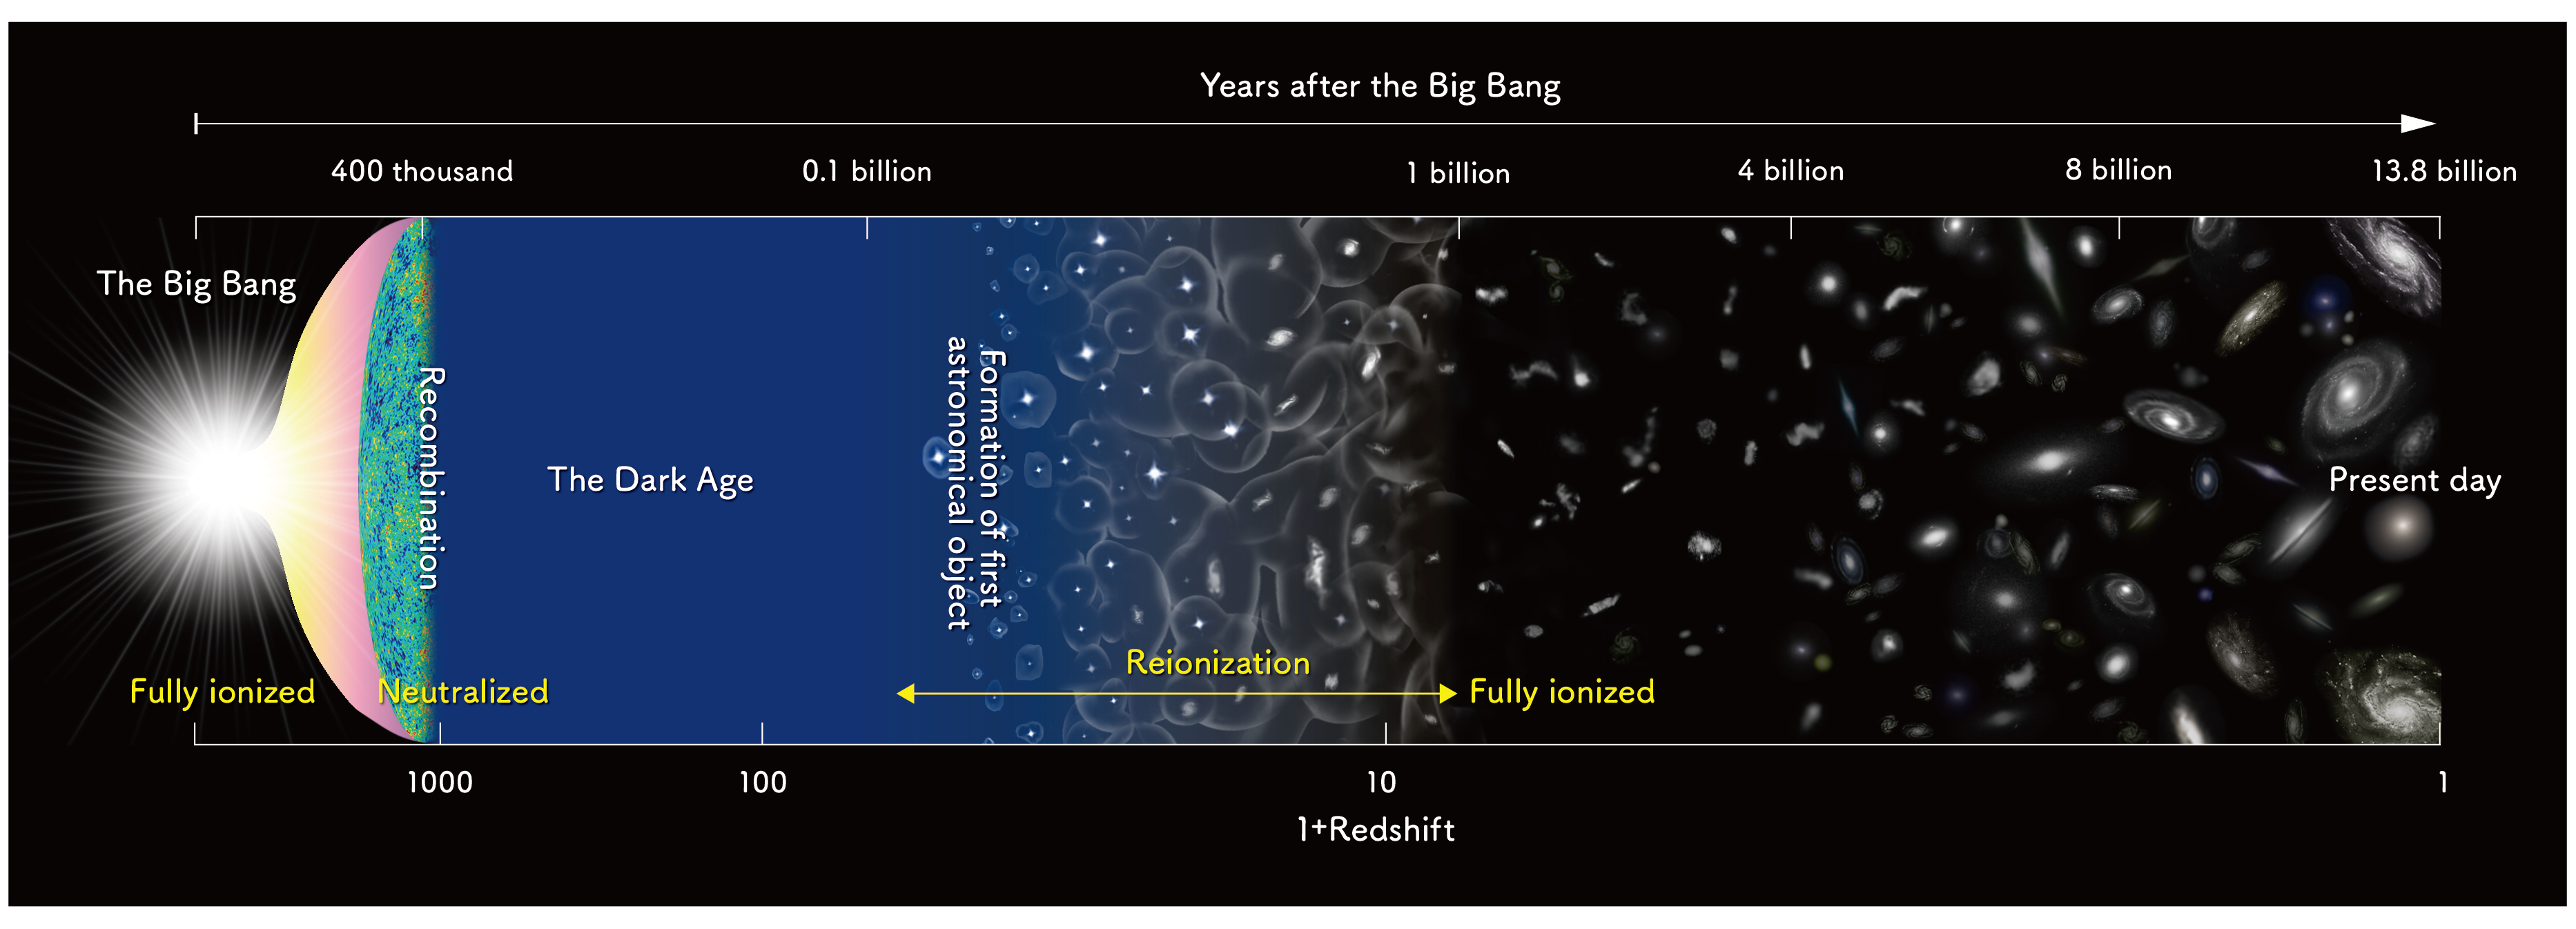
\includegraphics[width=\columnwidth]{plots/timeline_history.jpg}
	\caption{Timeline of the history of the Universe. The Epoch of Reionization marks the era when the first stars and galaxies formed and ionized the neutral hydrogen in the Universe. Image credit: NAOJ.}
	\label{fig:timeline_history}
\end{figure}

The exact timescale and details of the reionization process, which are shown within the context of the history of the Universe in Figure \ref{fig:timeline_history}, are current research questions in the field of cosmology. The physics of reionization depends on several factors, including the nature of the first stars (masses, luminosities, ionizing photons) and the surrounding gas (efficiency of the ionizing photons, feedback effects). There are several ways to approach the investigation of this era, with CMB measurements working to constrain the duration of reionization, galaxy measurements unveiling the end of reionization, and direct hydrogen measurements attempting to map out the changing nature of the gas over time. All of these probes serve to illuminate this watershed era between a Universe dominated by darkness and a Universe defined by light.

\subsection{CMB and Galaxy Measurements}

There are several observational probes of the reionization epoch, three of which we highlight in this section. The first is the study of CMB anisotropies, which carry with them an imprint of the early Universe. But that's not the only imprint it has - CMB photons can scatter off of free electrons after reionization, and these scatterings leave behind polarization and temperature imprints (\citealt{haiman_knox_1999}). For example, the amplitude of the CMB is sensitive to scatterings, as an increased number of scatterings is akin to mixing different parts of the CMB together as photons are scattered in all directions, or in other words, this scattering washes out anisotropies in the CMB and lowers its overall amplitude. 

A useful parameter to quantify the amount of electron scattering that occurs is the optical depth, $\tau_{es}$, defined as:

\begin{equation}
\tau_{es} = \int n_{e}\sigma_{T} dl,
\end{equation}
where $n_{e}$ is the number density of free electrons, $\sigma_{T}$ is the Thompson cross-section, and the integral is taken over a proper length $dl$. Once reionization begins, the number of free electrons increases, contributing to increasingly higher values of $\tau_{es}$. Hence, an earlier start for reionization would yield higher optical depths than a late reionization scenario. 

Observations of the CMB by WMAP and Planck have placed constraints on the optical depth parameter (\citealt{hinshaw_et_al2013}; \citealt{planck2016}), with the more recent Planck result suggesting a lower value of $\tau_{es} \sim 0.07$ than WMAP. This value suggests that reionization ends at a redshift of $z \sim 6$, with instantaneous reionization (``mean" reionization) at $z \sim 8.8$ (\citealt{planck2016}).

Currently, the results from CMB measurements are in agreement with a second powerful probe of EoR --- that is, observations of high-redshift galaxies. This probe comes in many flavors. For example, the spectra of distant quasars can illuminate the end of reionization. Quasars, being extraordinarily bright and energetic objects, are detectable at very far distances and their spectra reveal the amount of absorption their light has undergone due to neutral hydrogen. While nearby quasar spectra exhibit sharp absorption lines, distant ones show the Gunn-Peterson trough, implying that the quasar light was entirely suppressed by hydrogen absorption. Studying the absorption features of quasars at different redshifts implies that reionization has indeed ended by $z \sim 6$ (\citealt{becker_et_al2001}). 

In addition to quasar observations, high-redshift galaxy observations can also reveal important characteristics about the state of the intergalactic medium (IGM). Namely, distant star-forming galaxies can be detected using a variety of techniques, such as narrow-band imaging to find Lyman-$\alpha$ emitters (produced by recombination near young stars) or broad-band observations to find Lyman-break galaxies (spectral breaks associated with absorption by neutral hydrogen). High-redshift galaxy observations can then be used to construct luminosity functions (number of stars per luminosity interval) and star formation histories, which in turn impact the evolution of the IGM. 

More specifically, if star-forming galaxies dominated the reionization process, then the ionization rate can be related to star-formation parameters as:

\begin{equation}
\dot{n}_{\rm ion} = f_{\rm esc}\xi_{\rm ion}\rho_{\rm SFR},
\end{equation}
where $\dot{n}_{\rm ion}$ is the cosmic ionization rate, $f_{\rm esc}$ is the escape fraction of photons into the IGM, $\xi_{\rm ion}$ is the rate of production of ionizing photons for a stellar population, and $\rho_{\rm SFR}$ is the star formation rate density. All three parameters influence the rate at which the IGM is ionized, with the latter able to be constructed from galaxy luminosity functions. For example, \citet{robertson_et_al2015} used data from the Hubble Space Telescope to construct a star formation rate history out to high redshifts, backing out an optical depth parameter that is consistent with that of Planck. 

While galaxy measurements can be used to constrain the EoR, they are ultimately doing so by unveiling the properties of old, distant stars and galaxies. A similar, new technique that also aims to reconstruct the histories of the first luminous structures is observing nearby, metal-poor Local Group galaxies. Called ``galactic archaeology," observations of nearby star-forming ancestors can be used to constrain the faint-end slope of the luminosity function. Determining the shape of this function has important implications on the number of galaxies needed to drive reionization and the types of sources dominating this epoch (\citealt{weisz2017}). 

CMB measurements and galaxy observations are both important in studying the EoR. However, they each have their limitations. For example, CMB measurements can only reveal the integrated quantity of $\tau_{es}$, therefore unable to provide insight into the evolution of reionization as it progresses over time. Similarly, galaxy observations are currently hovering only around the tail end of the reionization era, and greater sensitivities are needed to push past this limit. A different, but complimentary, probe is needed to unlock the entire window into the EoR.

\subsection{Measurements of HI}

A direct measurement of neutral hydrogen gas over time would provide a fundamental way to track the IGM over the reionization process. Such a probe, which is made possible by the spin-flip transition of hydrogen, is a powerful technique that allows the tracing of gas over time, and it is this technique that serves as the basis for the remainder of this thesis (\citealt{furlanetto_et_al2006}; \citealt{barkana_and_loeb2008}; \citealt{morales_and_wyithe2010}; \citealt{pritchard_and_loeb2010}; \citealt{pritchard_loeb2012}). 

The spin-flip transition of neutral hydrogen occurs when a hydrogen atom changes energy state between two hyperfine levels. Namely, if a hydrogen atom moves from an aligned state to an anti-aligned state, the energy difference is released in the form of a photon with a wavelength of $21$\,cm. 

Because this transition has a well-defined wavelength, the signal can be directly mapped to a distance, or redshift, by measuring its wavelength upon detection. For example, a $21$\,cm photon that was initially emitted at a redshift of $z = 6$ would have expanded by a factor of ($1+z$) due to the expansion of the Universe and be $1.5$\,m long when it arrives at our telescopes. Hence, observing longer wavelengths of the hydrogen signal means that it has traveled for a greater distance (and has stretched out more) and thus comes from farther away at a higher redshift. This means that the $21$\,cm signal is a powerful tracer of 
neutral hydrogen at any distance (i.e. as a function of time), as long as it exists. This technique is especially compelling because it allows the direct exploration of the EoR as it occurs, whereas CMB measurements and galaxy measurements surround this era from the beginning and end only, respectively (Figure \ref{fig:timeline_circle}).

\begin{figure}
	\centering
	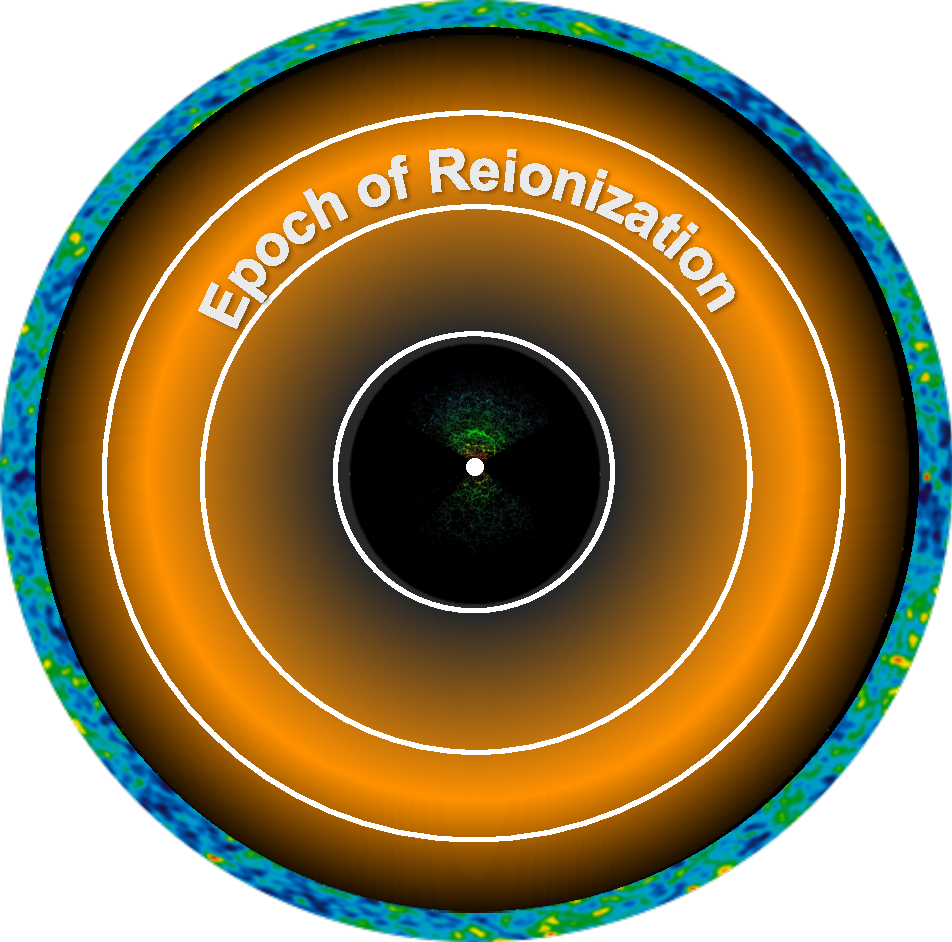
\includegraphics[width=0.5\textwidth]{plots/timeline_circle.pdf}
	\caption{A cartoon diagram of the observable Universe centered on us. Close-by, galaxy observations have mapped out cosmic web structure in our nearby Universe (image credit: SDSS). Far-away, the cosmic microwave background is observed at a redshift of $z \sim 1100$ (image credit: WMAP). The Epoch of Reionization represents a mostly unexplored era between the two, and can be probed by measuring red-shifted $21$\,cm radiation from neutral hydrogen.}
	\label{fig:timeline_circle}
\end{figure}

\begin{figure}
	\centering
	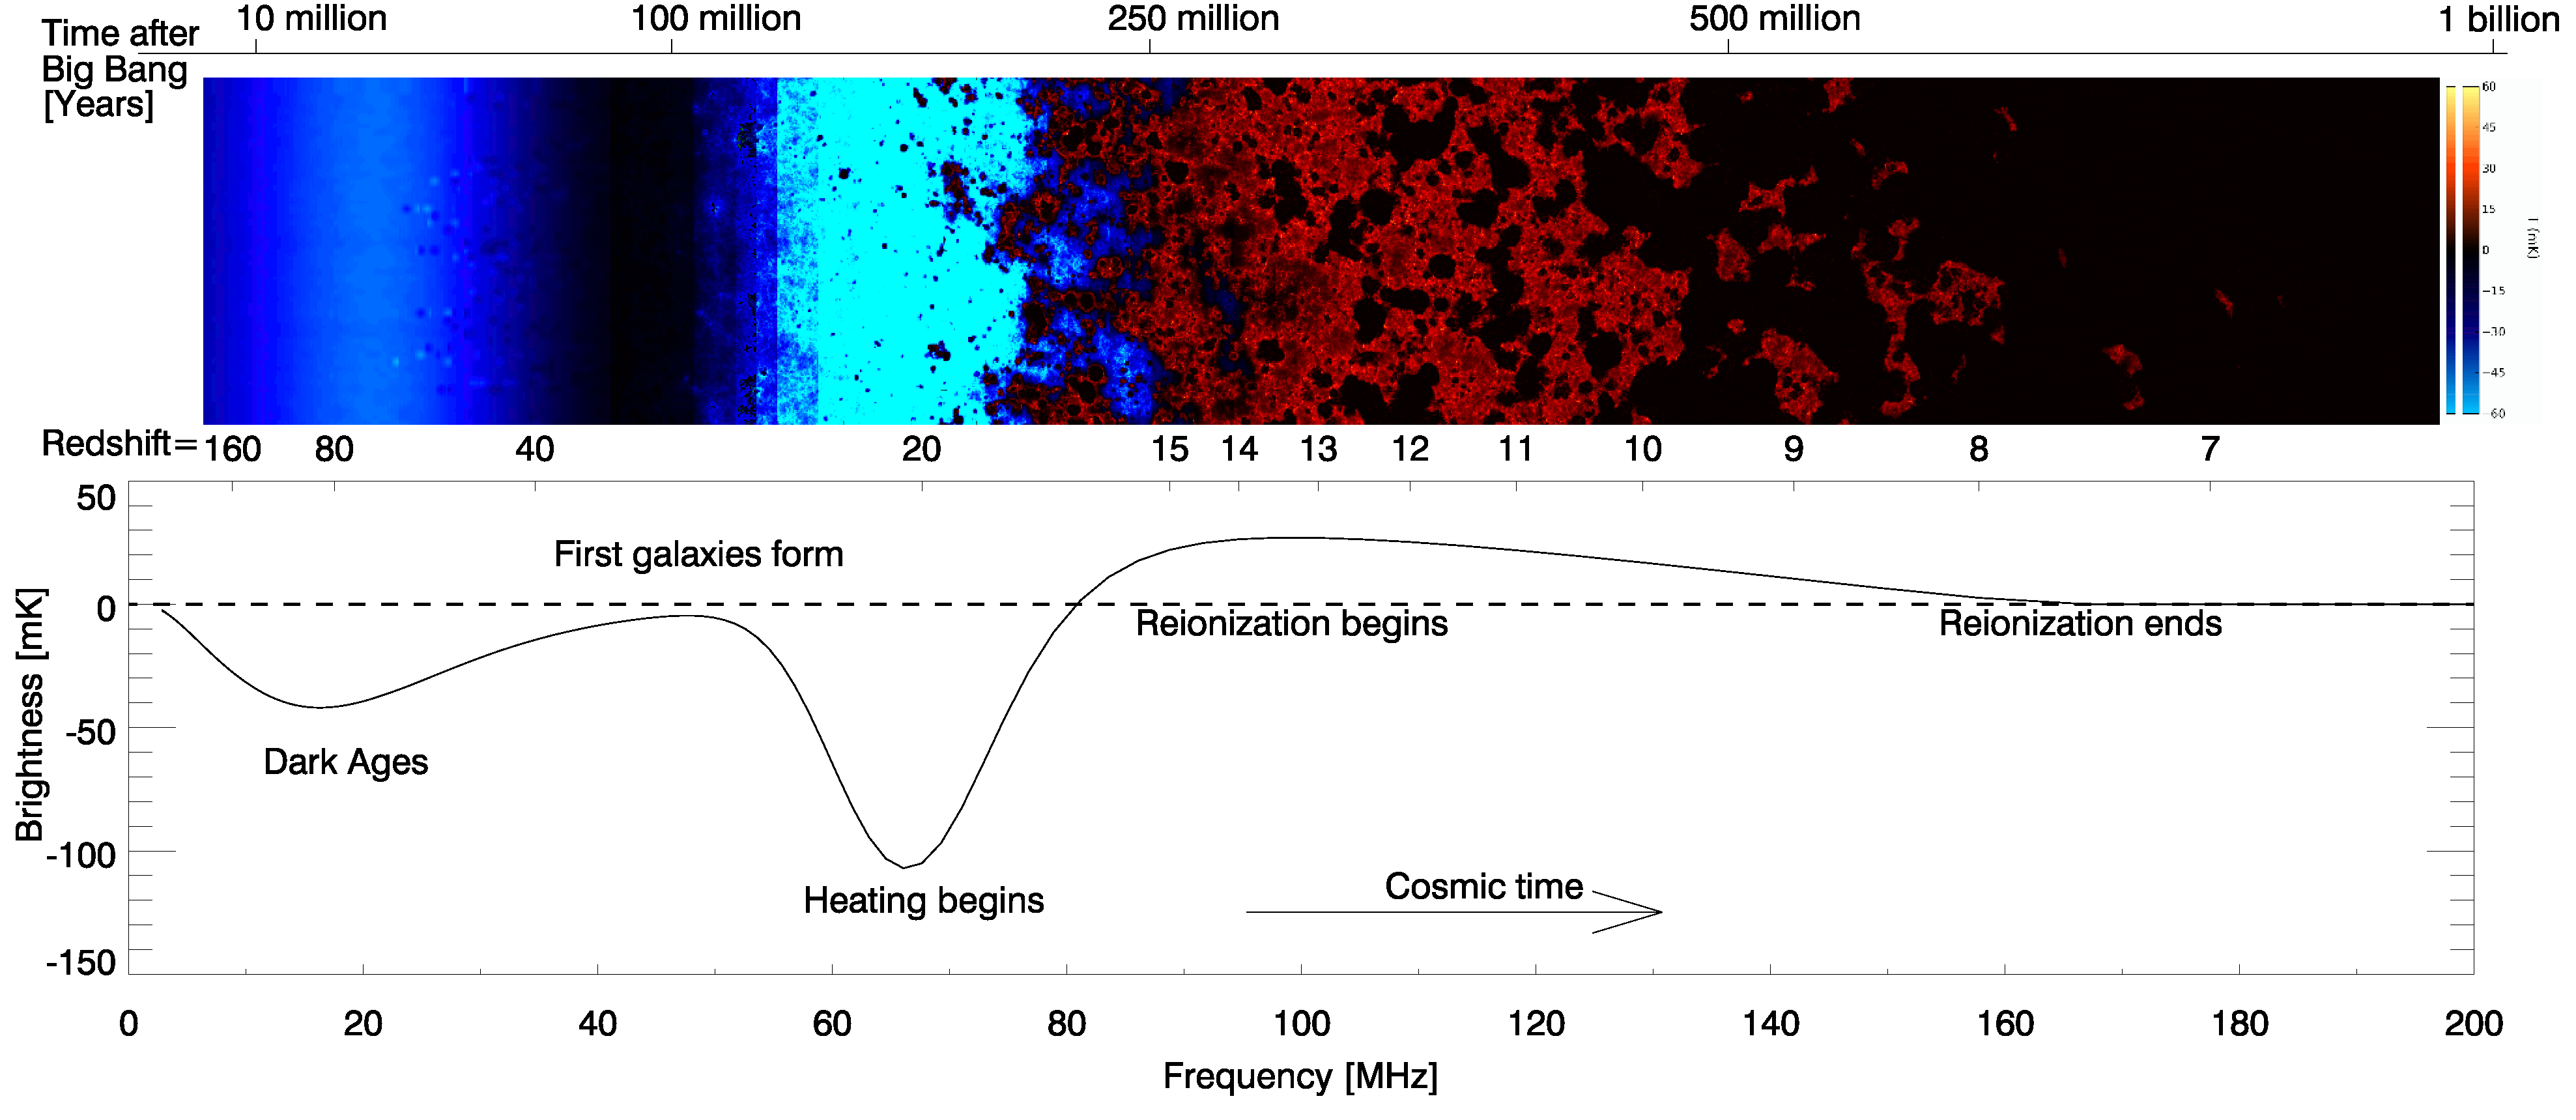
\includegraphics[width=\columnwidth]{plots/timeline_global.pdf}
	\caption{The evolution of the global $21$\,cm signal, starting with the Dark Ages, through galaxy formation and reionization (image credit: \citet{pritchard_loeb2012}). The work in this thesis mainly focuses on a redshift range of $6 < z < 12$ as reionization is expected to progress and complete.}
	\label{fig:timeline_global}
\end{figure}

In practice, the $21$\,cm signal is encapsulated by the quantity $T_{\rm spin}$, which measures the relative number of hydrogen atoms in the excited (aligned) versus ground (anti-aligned) spin-flip state. A high spin temperature means that the hydrogen gas is more likely to emit $21$\,cm photons, whereas a low $T_{\rm spin}$ implies that the gas is more likely to absorb $21$\,cm photons. 

The spin temperature is always measured with respect to the temperature of the CMB, which serves as a backlight for our measurement. During different stages of our cosmic history, $T_{\rm CMB}$ and $T_{\rm spin}$ take turns in the spotlight, with the \textit{differential brightness temperature}, $\delta T_{b}$ describing their evolution:

\begin{equation}
\label{eq:Tb}
\delta T_{b} \propto (1+\delta_{b})x_{HI}\Big(1-\frac{T_{\rm CMB}}{T_{\rm spin}}\Big).
\end{equation}
Equation \eqref{eq:Tb} captures the EoR signal that we would like to measure, where $\delta_{b}$ is the fractional over-density of matter and $x_{HI}$ is the fraction of neutral hydrogen ($1$ if all neutral, $0$ if all ionized). The differential brightness temperature can be measured in multiple ways --- in Chapter \ref{sec:interferometry} we explain how interferometry (many telescopes) can be used to measure the correlations of $\delta T_{b}$ on various spatial scales on the sky. Here we describe the evolution of the sky-averaged $\delta T_{b}$, called the \textit{global signal}, in order to summarize how the signal is expected to behave during our \textit{cosmic dawn} and through reionization.

A theoretical prediction for the evolution of $\delta T_{b}$ is shown in Figure \ref{fig:timeline_global}. At the very far left, a cool, neutral IGM remains after recombination and the release of the CMB. Residual electrons collide off of both CMB photons and the hydrogen gas, driving couplings between $T_{\rm gas}$ and $T_{\rm CMB}$, and $T_{\rm gas}$ and $T_{\rm spin}$, respectively. Hence, we expect to see no signal ($\delta T_{b} = 0$) at this time.

During the Dark Ages, collisions still couple $T_{\rm gas}$ and $T_{\rm spin}$, but Compton scattering becomes rarer as the CMB dilutes with the expansion of the Universe. While the CMB dilutes as $T_{\rm CMB} \propto 1/a$, where $a$ is the scale factor, the gas now follows an adiabatic expansion ($T_{\rm gas} \propto 1/a^{2}$). Thus, the gas cools quicker than the CMB, and since it is still coupled to the spin temperature, $T_{\rm spin} < T_{\rm CMB}$ and the signal is expected to be seen in absorption. By the time the first galaxies begin forming, however, the gas is expected to be so dilute that it is no longer coupled to the spin temperature. The spin temperature therefore couples once again to the CMB, and no signal is produced.

As the first stars in the first galaxies begin emitting Lyman-$\alpha$ photons, the hydrogen gas is excited and de-excited, coupling $T_{\rm spin}$ and $T_{\rm gas}$. The gas, still cool from adiabatic expansion, implies that $T_{\rm spin} < T_{\rm CMB}$ and the signal is seen in absorption. Eventually, x-rays from the first sources begin heating the cooled gas, driving both the gas and spin temperatures above that of the CMB, where the signal is expected to be seen in emission for the first time. 

Finally, even though the timing and details of reionization are unknown, UV photons from the first luminous structures are believed to eventually ionize all the neutral hydrogen, leaving no signal to be detected by a redshift of $z \sim 6$. 

The shape of the global signal holds important science implications about our early Universe. For example, the position of the heating trough reveals the types of sources and energies of the x-rays doing the heating, as well as the sizes of the dark matter halos hosting those first sources (i.e. late heating and deep absorption troughs imply harder x-ray spectras, as shown in \citet{fialkov_et_al2014}). The first tentative detection of this signature from the Experiment to Detect the Global Epoch of Reionization Signature (EDGES) even suggests that known physics and commonly accepted scenarios may not be responsible for creating the absorption profile (\citealt{bowman_et_al2018}). As the field continues to investigate our cosmic dawn through HI measurements --- both the global signal and statistical fluctuations ---  we can expect to learn much about the constituents that make up the Universe and their complex interactions during this era.

\subsection{This Thesis}

Although $21$\,cm observations promises an uninterrupted window into the EoR, from which we can learn much about galaxy formation and the properties of the IGM, there are many challenges facing this field of cosmology. In general, the $21$\,cm signal is extremely faint, with bright foregrounds (mostly synchrotron radiation from our own Galaxy) and radio interference easily overshadowing the target signal. As a consequence, instruments need to be extremely well-understood, precisely calibrated, and capable of being sensitive enough for a successful detection. In addition, analysis techniques must be innovative and rigorously construed so as to be able to extract clean and accurate measurements.

In this thesis, I present work associated with data from radio interferometers seeking to measure $21$\,cm fluctuations during the EoR. While a confirmed detection by an interferometer remains elusive at this time, this work serves as a huge leap forward in working with large datasets and extracting measurements of the cosmological signal with confidence. The rest of this thesis thus focuses on the characterization of data from large telescope arrays in order to place accurate, stringent limits on the EoR signal. It is an exciting time and this field is young, and the work in this thesis serves as a foundation of what promises to be an eye-opening adventure to-come.

\section{Interferometry}
\label{sec:interferometry}

Multiple radio telescopes (i.e. an interferometer) can be used in combination to probe $21$\,cm fluctuations. A pair of antennas receives sky signal at slightly different times, with a time delay determined by the antenna spacing, or baseline orientation and length. The two voltage streams from the antennas are then correlated, with the output response having an amplitude dependent on the sky's flux density and a phase dependent on the time delay between the two elements and the frequency of the light. In other words, every pair of antennas of an interferometer measures an interference pattern, and knowledge of the entire sky can be built up by having a large number of antennas and many different types, and copies, of baselines.

\subsection{The Visibility Equation}

The output measurement from correlating signals between two antennas is called a \textit{visibility}. The visibility can be written as:

\begin{equation}
\label{eq:vis}
V_{ij}(\nu) = S(\nu) e^{-2\pi i\frac{\vec{b}_{ij}\cdot \hat{s}}{\lambda}},
\end{equation}
where $i,j$ represent a pair of antennas, $S(\nu)$ is the sky flux density, $\vec{b}_{ij}$ is a baseline vector, $\hat{s}$ is a unit-vector in the direction of a source in the sky, and $\lambda$ is the wavelength of the signal. The fractional term in the exponential reflects the changing number of wavelengths between the two antennas as a signal goes in and out of phase as the source passes overhead, for example. The entire exponential term represents the phase of the visibility, which can also be described as the fringe pattern, or diffraction pattern, between two antenna elements. 

Equation \eqref{eq:vis} represents a visibility measurement for one time integration and one direction on the sky. In practice, we compute the integrated visibility over the entire angular sky $d\Omega$:

\begin{equation}
V_{ij}(\nu,\Omega) = \int A(\nu,\Omega)I(\nu,\Omega) e^{-2\pi i\frac{\vec{b}_{ij}\cdot \hat{s}(\Omega)}{\lambda}}d\Omega,
\end{equation}
where the amplitude component has been broken up into a primary beam component $A(\nu,\Omega)$ and sky flux density component $I(\nu,\Omega)$. The primary beam describes the power pattern of an antenna element and determines its field of view, thus altering the power received from the sky depending on its direction.

The visibility equation can be re-interpreted as the 2-dimensional Fourier-transform of the sky. In other words, the Fourier-transform of a visibility produces a \textit{dirty image} of the sky, from which the true sky can be reconstructed by de-convolving out information from the antenna beam. 

In this thesis, we focus on cross-correlations, or power spectral measurements, of visibilities. Recalling that we seek to measure the differential brightness temperature on various spatial scales of the sky, we can form the quantity:

\begin{equation}
\langle \delta \tilde{T}_{b}(\vec{k})^{\ast} \delta \tilde{T}_{b}(\vec{k})\rangle = (2\pi)^{3} \delta^{D}(\vec{k}-\vec{k}')P_{21}(\vec{k}) ,
\end{equation}
where $\delta \tilde{T}_{b}(\vec{k})$ is the Fourier-transform of the differential sky brightness as a function of cosmological wavenumber $\vec{k}$ (i.e. our visibility measurement, up to scaling factors), $\delta^{D}$ is the Dirac-delta function, and $P_{21}$ is the $21$\,cm power spectrum quantity we are interested in eventually forming.

Simply speaking, because our visibility measurements have already taken two spatial Fourier-transforms out of the three needed for a 3D power spectrum, we need only to take one last Fourier-transform (along frequency), and then multiply and average the visibilities together for a given baseline in order to compute a power spectral measurement. Having repeated baseline copies then increases the sensitivity to a given Fourier-mode on the sky, while having different types of baselines makes it possible to measure multiple Fourier-modes and build up an image of the sky. Since the EoR signal is expected to be present everywhere on the sky, in this work we focus on the former technique in order to maximize our sensitivity to the cosmological signal.

The last thing to note is that the wavenumber $\vec{k}$ can be broken up into a perpendicular component $\vec{k}_{\perp}$ and a parallel component $k_{\parallel}$, where $\vec{k}_{\perp}$ is proportional to the (x,y) spatial coordinates on the sky and $k_{\parallel}$ is proportional to the line-of-sight direction on the sky (i.e. frequency). Every unique baseline probes a single $\vec{k}_{\perp}$, and it's worth noting that, because we focus on redundant baselines in the analysis to follow, most of our power spectrum sensitivity comes from the frequency-direction. Accounting for cosmological distance, a 1D wavenumber has units of Mpc$^{-1}$, so that the 3D power spectrum has units of mK$^{2}\cdot$Mpc$^{3}$. Visibility measurements typically have units of Janskys.

\subsection{Calibration}
\subsection{Foreground and Filtering}
\subsection{Fringe-rate Filtering}

\section{Instruments}
\subsection{The Precision Array for Probing the Epoch of Reionization}
\subsection{The Hydrogen Epoch of Reionization Array}
\subsection{Other Experiments}

%\nocite{*}






